\documentclass{article}
\usepackage[top=1in,bottom=1in]{geometry}
\usepackage{hyperref}
\usepackage{amsmath}
\usepackage{amssymb}
\usepackage{graphicx}
\graphicspath{ {./assets/} }
\usepackage[none]{hyphenat}
\usepackage{listings}
\usepackage{color}
\definecolor{dkgreen}{rgb}{0,0.6,0}
\definecolor{gray}{rgb}{0.5,0.5,0.5}
\definecolor{mauve}{rgb}{0.58,0,0.82}
\lstset{frame=tb,
  language=C,
  aboveskip=3mm,
  belowskip=3mm,
  showstringspaces=false,
  columns=flexible,
  basicstyle={\small\ttfamily},
  numbers=none,
  numberstyle=\tiny\color{gray},
  keywordstyle=\color{blue},
  commentstyle=\color{dkgreen},
  stringstyle=\color{mauve},
  breaklines=true,
  breakatwhitespace=true,
  tabsize=3
}
\date{}
\title{CMSC417 Computer Networks}
\begin{document} 
  \author{Michael Li}
  \title{CMSC417 Computer Networks}
  \maketitle
  \tableofcontents
  \newpage
  \section{Foundations}
  \subsection{Requirements}
  \textbf{Requirement 1: Scalable Connectivity}: Network should be scalable and should be able to connect to connect to a lot of devices. At the lowest level, \textbf{nodes} (computers) are connected by \textbf{links} (e.g. wire).
  \begin{itemize}
    \item \textbf{Point-to-point}: link is only shared between 1 pair of nodes
    \item \textbf{Multiple-access}: link is shared between several nodes
  \end{itemize}
  \textbf{Indirect connectivity}: can be achieved in multiple ways:
  \begin{itemize}
    \item \textbf{Switched network}: uses nodes that forward data received from one link and out the other link.
      \begin{itemize}
        \item \textbf{Circuit switched}: establishes a stream of bits
        \item \textbf{Packet switched}: nodes send blocks of data in the form of \textbf{packets} and use \textbf{store-and-forward} where the node has to receive entire packet, storing it in memory, before forwarding the entire packet. Here the \textbf{switches} implement the network and the \textbf{hosts} use the network
      \end{itemize}
    \item \textbf{Internetwork (internet)}: set of independent networks connected by \textbf{routers} that are nodes that act like switches between networks.
  \end{itemize}
  In order to provide \textbf{host-to-host} connectivity, each node is assigned an \textbf{address} that allows other nodes to communicate with the node. Switches and routers use this address to \textbf{route} messages to their destination \\ \\
  \textbf{Requirement 2: Efficiency} \\
  \textbf{Multiplexing}: system resources shared among multiple users. Achieved by using
    \begin{itemize}
      \item \textbf{Synchronous Time Division Multiplexing (STDM)}: divide time into equally sized chunks and round-robin each flow
      \item \textbf{Frequency Division Multiplexing (FDM)}: transmit each flow at different frequencies
      \item STDM and FDM both have issues in that links may be idle during a given time interval or at a particular frequency. Also, both do not support adding new flows easily.
      \item \textbf{Statistical Multiplexing}: links are shared on a time-basis but is on demand, rather than a predetermined time slot. Also limits the size of packets sent over to ensure data is not lost.
    \end{itemize}
    With multiplexing, switches may need to buffer packets if the input rate $>$ output rate. This can lead to \textbf{congestion} where the buffer is full so it needs to drop packets \\ \\
    \textbf{Requirement 3: Support for Common Services}: networks provide \textbf{logical channels} that application processes use to communicate with each other. These channels provide a set of services and are typically imlpemented on end hosts to keep links simple \\ \\
    \textbf{Requirement 4: Reliability}: need to consider 3 types of errors
    \begin{itemize}
      \item \textbf{bit error}: bit is flipped in the physical link
      \item \textbf{packet loss}: packet is dropped or uncorrectable packet is discarded
      \item \textbf{physical crash}: e.g. network shutsdown
    \end{itemize}
  \textbf{Requirement 5: Managbility}: system needs to be scalable (should be able to support more devices)
  \subsection{Network Architecture}
  \textbf{Network Architecture} is a blueprint that guides the design and implementation of networks. Uses \textbf{layering} and \textbf{abstraction} to capture the important aspects of a system. Services at higher \textbf{protocols} (layers) are built using the services of the lower protocols. These protocols define 2 different interfaces:
  \begin{itemize}
    \item \textbf{service interface}: defines operations local objects can perform on the protocol (e.g. sending and receiving messages)
    \item \textbf{peer interface}: defines the form and meaning of messages exchanged between protocol peers
  \end{itemize}
  \textbf{Peer-to-peer interaction} is indirect; each protocol communicates with its peer by passing messages to lower level protocols that deliver the messages to its peer. This ends up creating a \textbf{protocol stack}. On the peer side, protocol layers are popped until we reach the original target. \\ \\
  \textbf{Encapsulation} is performed at each protocol level; \textbf{headers} are attached to the \textbf{payload} (rest of the message) and instruct the peer on how to handle the message (i.e. how the payload is passed to the next higher level in the peer). \\ \\
  A \textbf{demux key} is attached to the header, allowing protocols to demultiplex messages to the correct application on the destination host
  \begin{center}
    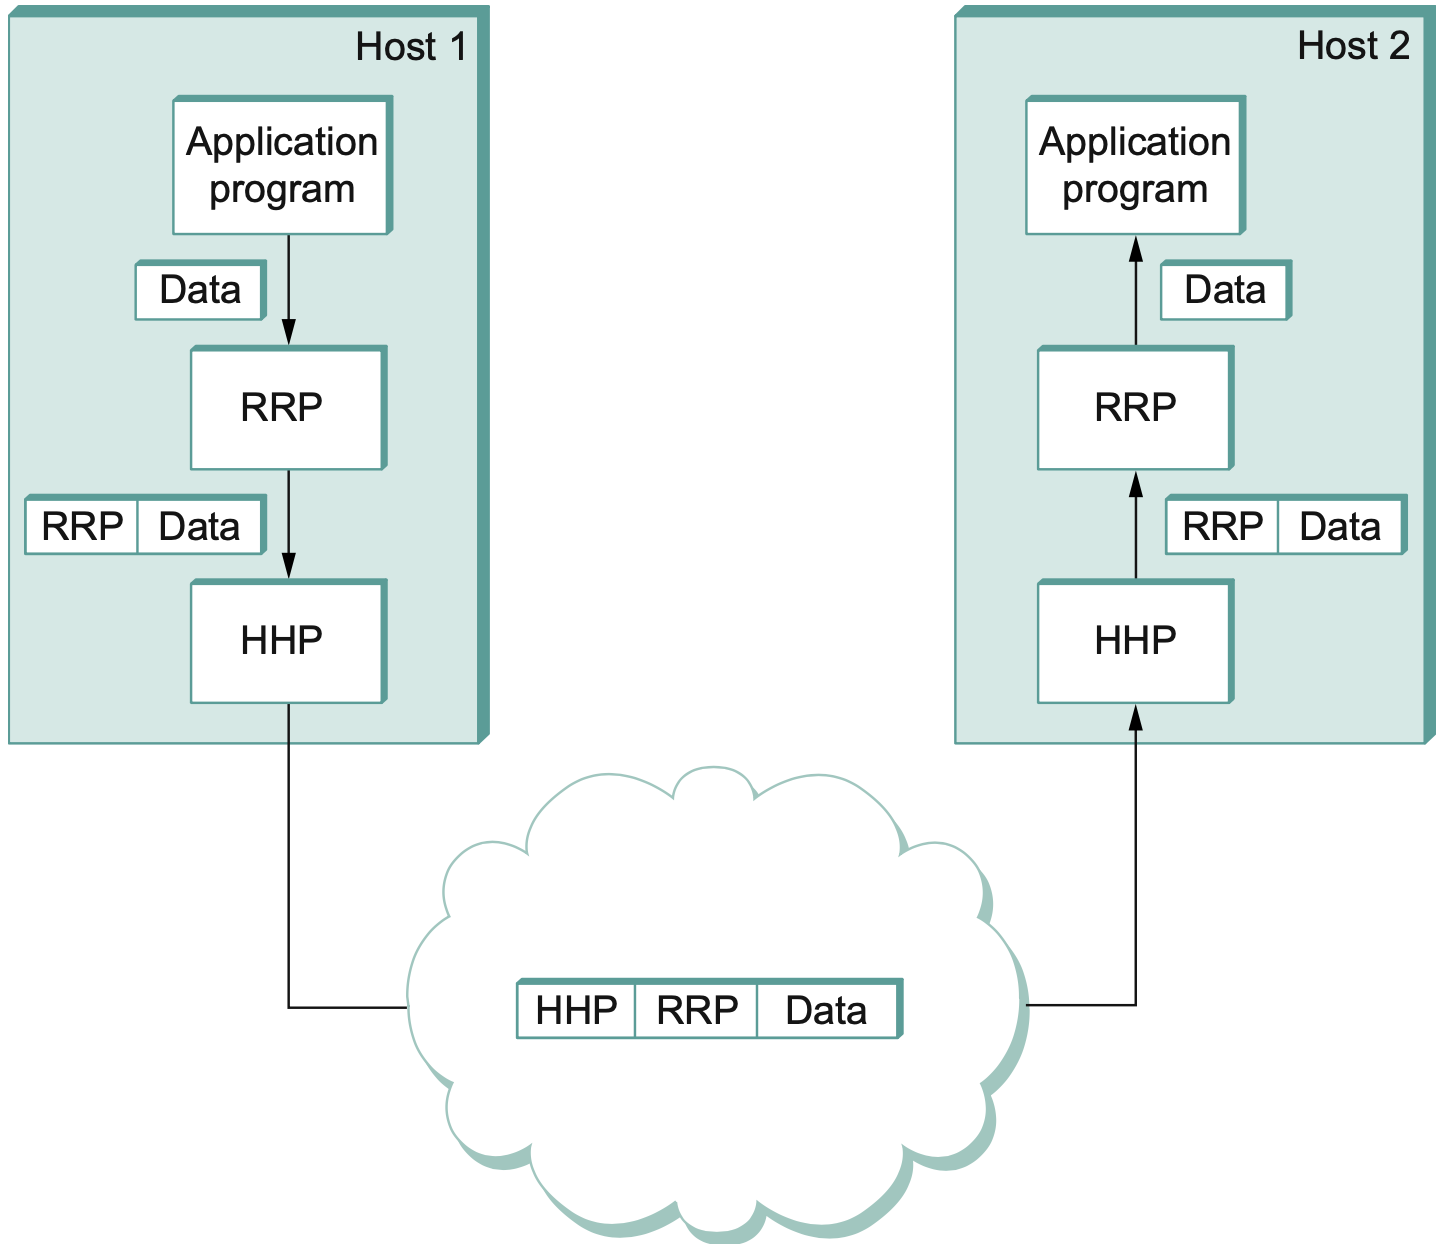
\includegraphics[scale=0.3]{Encapsulation.png}
  \end{center}
  \textbf{Open Systems Interconnection (OSI)}: partitions network functionality into 7 layers
    \begin{itemize}
      \item \textbf{Physical layer}: handles transmission of raw bits over communication link
      \item \textbf{Data link layer}: aggregates bits into \textbf{frames}
      \item \textbf{Network layer}: routes packets to nodes within packet-switched network. Unit of data exchanged is called \textbf{packet}
      \item \textbf{Transport layer}: implements process-to-process channels that exchange messages. Unit of data here is called \textbf{messages}
      \item \textbf{Session layer}: ties potentially different transportation streams
      \item \textbf{Presentation layer}: concerned with the format of data being exchanged
      \item \textbf{Application layer}: handles high level protocols
    \end{itemize}
  \begin{center}
    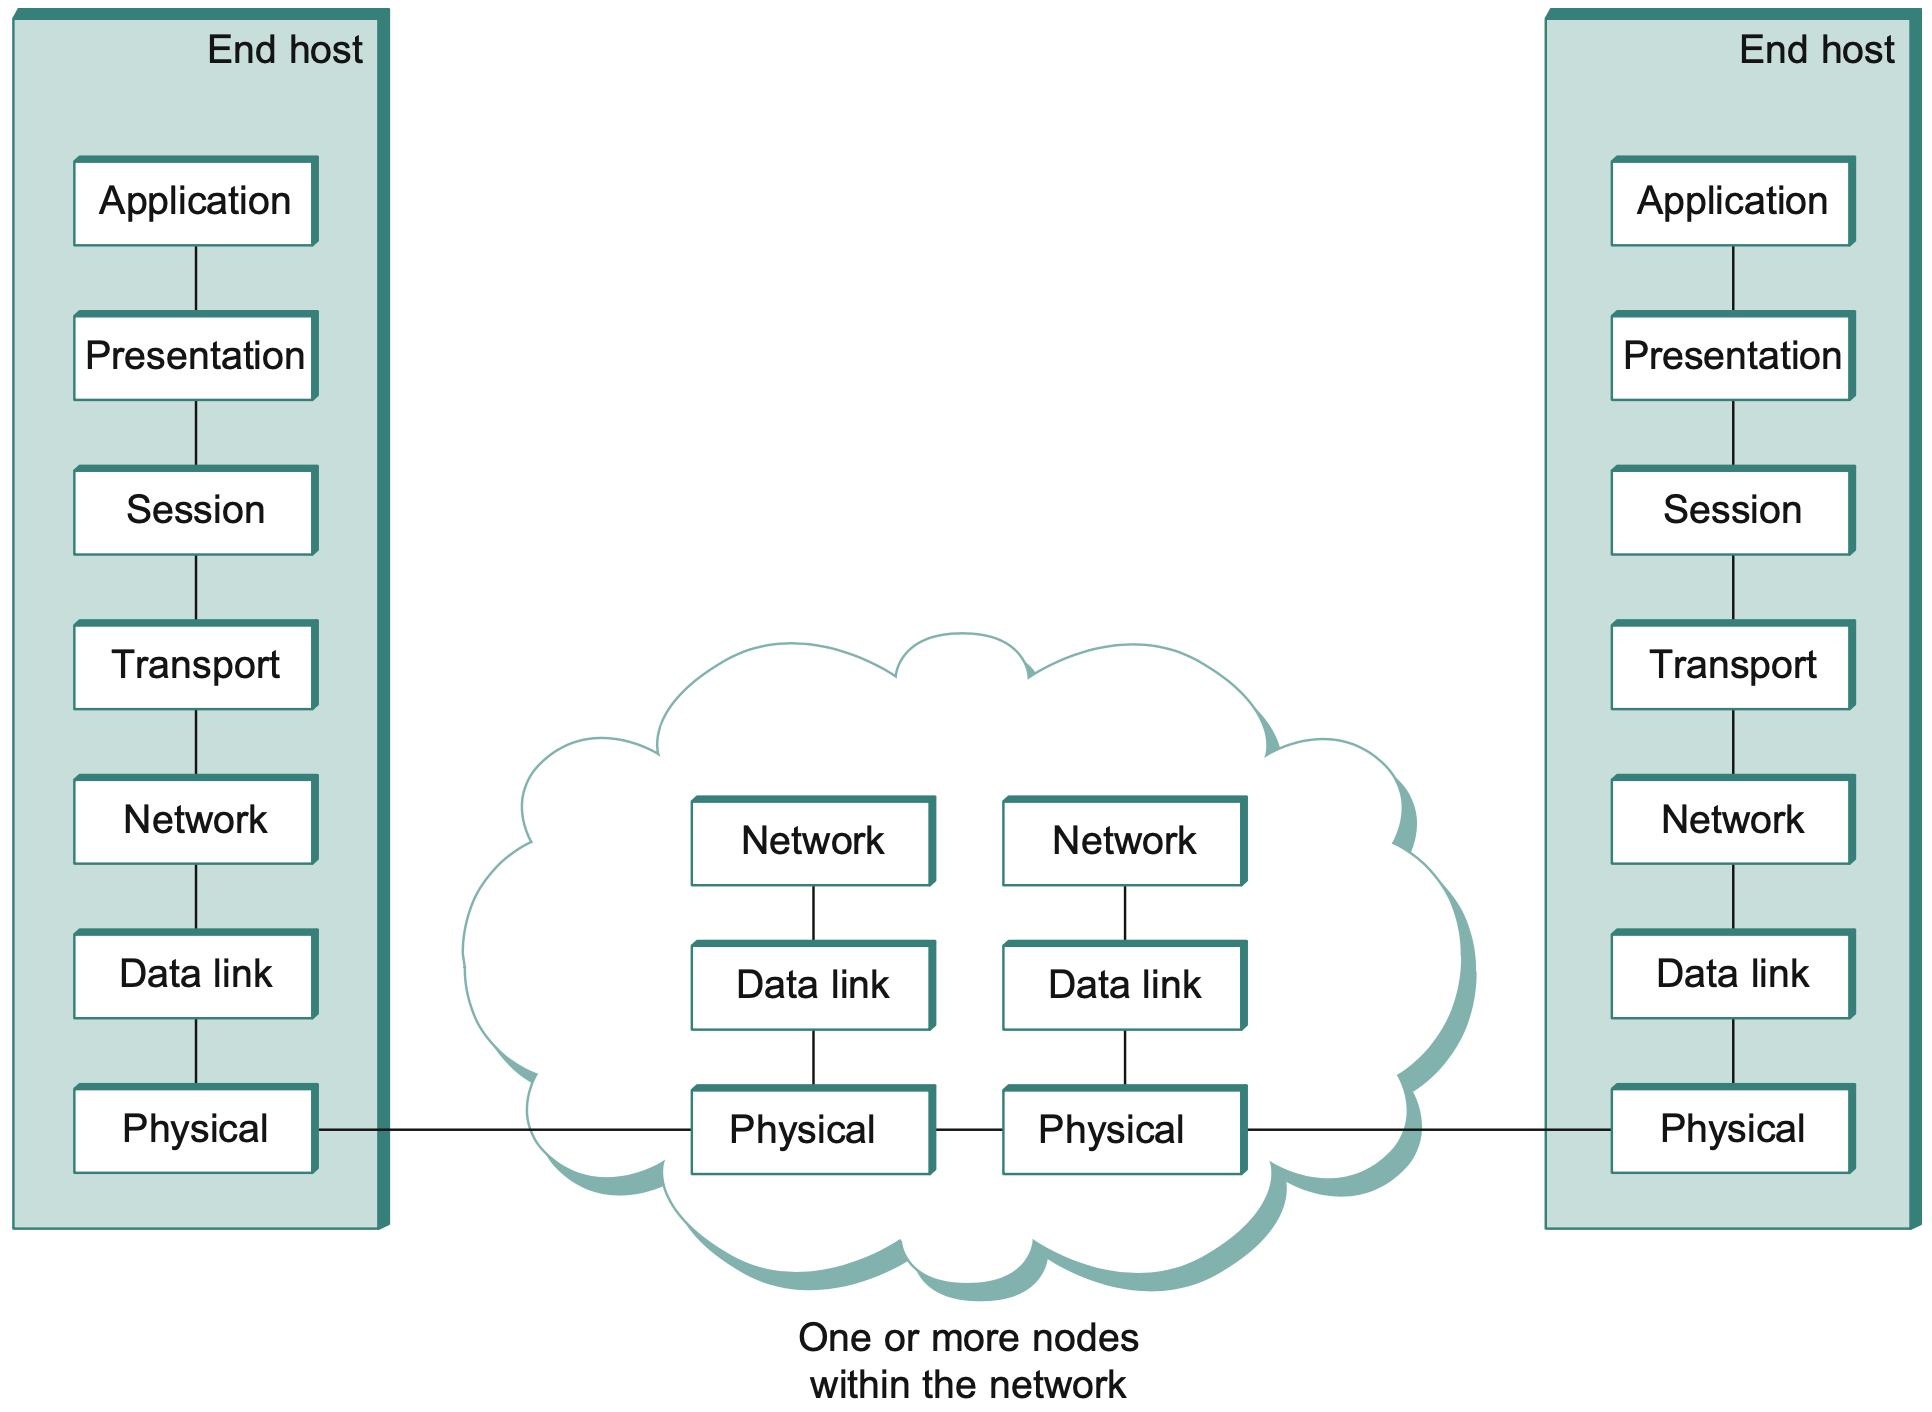
\includegraphics[scale=0.25]{OSI}
  \end{center}
  \textbf{Internet Architecture}: 4 levels:
    \begin{itemize}
      \item \textbf{Network protocols}: lowest leevel implemented by a combination of hardware and software
      \item \textbf{Internet protocol (IP)}: supports multiple networking technologies into 1 internetwork
      \item \textbf{Transmission control protocol (TCP)} and \textbf{User Datagram Protocol (UDP)}: TCP provides reliable byte-stream channel and UDP provides unreliable datagram delivery channel
      \item \textbf{Application protocols}: enable interoperation of applications
      \item One main difference between Internet Architecture and OSI is that layering isn't prevelant for the former; apps can skip layers if desired
    \end{itemize}
  \begin{center}
    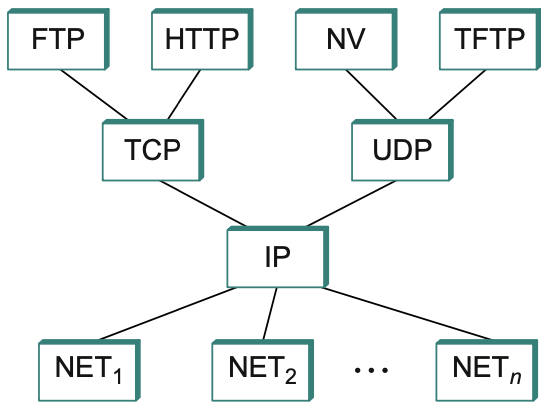
\includegraphics[scale=0.5]{InternetArchitecture}
  \end{center}
  \subsection{Implementing Network Software}
  \textbf{Socket}: the point where application attaches to the network. The interface defines how to create sockets, how to attach them to network, how to send and receive messages through sockets, and how to close sockets. To create a socket in TCP:
    \begin{itemize}
      \item invoke socket() to create socket
      \item for the server side, perform a \textbf{passive open} (prepared to accept connections but doesn't actually establish them) by invoking bind(), listen(), and accept()
      \item for the client side, perform an \textbf{active open} (says who it wants to communicate with) by invoking connect(). Once connected, can invoke send() and recv() to send and recieve messages from specified socket to a buffer
    \end{itemize}
\begin{lstlisting}
// domain: protocol family
// type: semantics of communication
// protocol: procol used
// returns a handle (identifier for socket)
int socket(int domain, int type, int protocol);

// binds created socket to a specific address
int bind(int socket, struct sockaddr *address, int addr len)
// listen defines how many connections can be pending on a socket
int listen(int socket, int backlog)
// accept carries out passive open
int accept(int socket, struct sockaddr *address, int *addr len)

// connect doesn't return until TCP has established a connection
int connect(int socket, struct sockaddr *address, int addr len)
// once connection is established, applications can send and recieve messages
int send(int socket, char *message, int msg len, int flags)
int recv(int socket, char *buffer, int buf len, int flags)
\end{lstlisting}
  \subsection{Network Performance}
    Performance measured by \textbf{bandwidth} (number of bits transmitted over time) and \textbf{latency} (how long it takes for message to travel) \\ 
    Bankwidth can be broken down into a sum of 
    \begin{itemize}
      \item speed of light propogation (distance/S)
      \item time to transmite a unit of data (size/bandwidth)
      \item queuing delays
    \end{itemize}
    \textbf{Delay $\times$ bandwidth product}: maximum number of bits that can travel in a pipe at once. Tells how many bits must be set before first bit arrives at receiver
  \section{Routing}
  \subsection{Vocabulary}
  \textbf{Forwarding (Data Plane)}: receiving a packet, looking up its destination on a table, and sending the packet in the appropriate direction. \\
  \textbf{Routing (Control Plane)}: process that builds \textbf{forwarding tables}. \\
  \textbf{Forwarding table}: contains information regarding mappings from network prefix to an outgoing interface to aid in forwarding packet. \\
  \textbf{Routing table}: contains mappings of network prefixes to next hops. \\
  \textbf{Routing domain}: internetwork where all routers are under the same administrative control.
  \subsection{Network as a Graph}
  Entire network can be represented as a graph (nodes, network links as edges with cost). The goal of \textbf{routing} is to find the lowest-cost path between any 2 nodes. Algorithms that calculate the shortest path usually do so in a dynamic, distributed manner, but this can lead to some confusion when different paths thinking that they have the shortest path available. There are 2 main routing protocols: \textbf{Distance vector} and \textbf{Link state}.
  \subsubsection{Distance Vector}
  Each node constructs an array (vector) that contains the cost to all other nodes and distributes this vector to its immediate neighbor and the vector is updated based on which nodes can be reached by the neighbor node. Links that are down are assigned an infinite cost.
  \begin{center}
    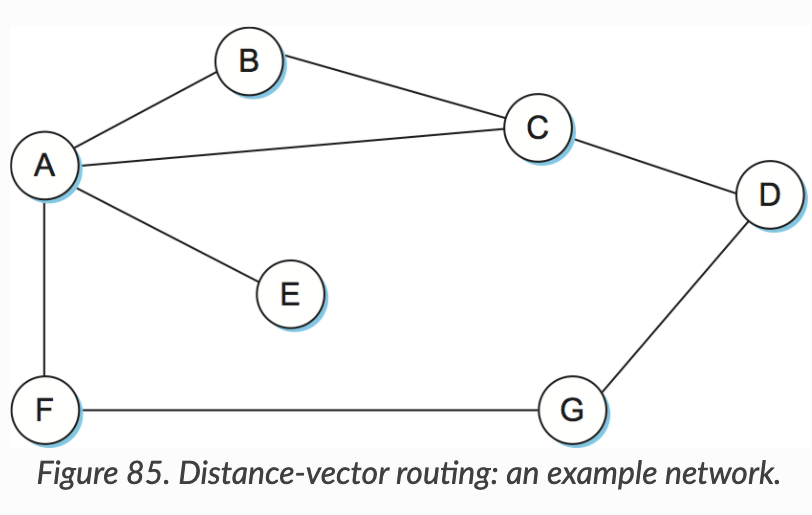
\includegraphics[scale=0.5]{DistanceVector}
  \end{center}
  Each routing tables contains entries (destination, cost, next hop). Routers exchange information (destination, cost) with immediate neighbors and the table is built from a sequence of exchanges. \textbf{Note}: nodes propagate a global view to its neighbors.\\ \\
  End result is that each node has the same routing table so routing information is consistent (\textbf{convergent}). Note that no one node contains all information in this table, each node only knows about the content of its own routing table. There are 2 ways in which updates occur:
  \begin{itemize}
    \item \textbf{Periodic update}: each node automatically sends an update message, even if nothing has changed, to let other nodes know that it is still running and to allow other nodes check if the current route becomes unviable.
    \item \textbf{Triggered udpate}: occurs when a node notices a link failure or receives an update from one of its neightbors that causes 1 of the routes in the routing table to change. This then triggers an update to the node's other neighbors.
  \end{itemize}
  \textbf{Count to infinity} problem: example - from the graph above, if the link A to E goes down, A notifies its neighbors that its distance to E is infinity, but B and C claim that they have a distance of 2 away from E. This then leads to the conclusion that A is 3 away from E, and then B and C is 4 away, leading to a distance of infinity. Potential solutions include:
  \begin{itemize}
    \item Set a maximum (e.g. 16) to represent infinity. Once we reach that many hops, we claim that the distance is infinity. This solution is restrictive in that it isn't scalable.
    \item \textbf{Split horizon}: when a node sends updates, it does not send routes it learned from a specific neighbor to that same neighbor. However, this solution isn't scalable for loops involving more than 2 nodes.
    \item \textbf{Poisoned reverse}: report failed links as $\infty$ which helps with routing loops involving 2 nodes. Doesn't work well loops involving $\geq 2$ nodes.
  \end{itemize}
  \textbf{Routing Informatoin Protocol (RIP)}: canonical example of routing protocol built on distance vector algorithm
  \subsubsection{Distance Vector Notations}
  $x.C(y)$ link cost from node $x$ to node $y$. If they are not neighbors, value is $\infty$ \\
  $x.D(z \rightarrow y)$ distance known to $x$ to travel from $z$, a neighbor of $x$, to $y$ \\
  $x.N$ set of neighbors to $x$ \\
  $\mathbb{N}$ set of all nodes \\
  $x \rightarrow y : M$ node $x$ sends a message $M$ to $y$ \\
  At the start, routing table consists of values:
  \begin{itemize}
    \item if $y \in x.N$ \implies $x.D(y \rightarrow y) = x.C(y)$
    \item if $y \notin x.N \implies \forall v \in x.N, x.D(v \rightarrow y) = \infty$
  \end{itemize}
  Entries consist of:
  \begin{itemize}
    \item destination
    \item cost
    \item next hop
  \end{itemize}
  At the end, routing table consists of values:
  \begin{itemize}
  \item $\underbrace{x.D(z \rightarrow y)}_{z \in x.N} = x.C(z) + \underbrace{\min}_{v \in z.N}(z.D(v \rightarrow y))$
  \end{itemize}
  \subsubsection{Distance Vector Protocol}
  $x$ sends an update message, $M = \forall d \in \mathbb{N}, (d, \underbrace{\min}_{v \in x.N}(x.D(v \rightarrow d)))$, to all $v \in x.N$ \\ \\
  When $x$ receives update from neighbor $v$:
  \begin{itemize}
    \item Did $x.C(v)$ change? If yes, $\forall y \in \mathbb{N}, x.D(v \rightarrow y) = \underbrace{x.D(v \rightarrow y) + \delta}_{\text{old val + change}}$
      \begin{itemize}
        \item Did the lowest cost to $y$ change? If yes, update the routing table.
      \end{itemize}
    \item Did $\underbrace{\min}_{z \in v.N}(v.D(z \rightarrow y))$ (best distance from $v \rightarrow y$) change?\\ 
      If yes, update $x.D(v \rightarrow y) = \underbrace{x.C(v) + \delta}_{\text{link cost + new change}}$
      \begin{itemize}
        \item Did the lowest cost to $y$ change? If yes, update the routing table.
      \end{itemize}
  \end{itemize}
  \subsubsection{Link State}
  Since each node knows how to reach its neighbors, we can make it so that this information is known to each node to create a complete map of the network at each node. \textbf{Note}: nodes propagate local views to all nodes so each has enough information to compute routes locally and can detect routing loops from failures. Relies on
  \begin{itemize}
    \item \textbf{Reliable flooding}: making sure that all nodes get the same copy of the link-state information from all the other nodes. Nodes send their link-state information (\textbf{link-state packet (LSP)}) to all of their neighbors who then forward to their neighbors until all nodes have been reached. LSPs contain
      \begin{itemize}
        \item ID of node that created the LSP
        \item list of connected neighbors of that node with the link cost to each one
        \item sequence number
        \item time to live for this packet
      \end{itemize}
      First 2 items enable route calculation. Last 2 items make flooding more reliable (ensuring that each node has the most recent copy of the information since there might be multiple LSPs from different nodes traversing the network) \\ \\
      Nodes receive \textbf{ACK} (acknowledgement) packets when they send an LSP. The LSP is retransmitted if no ACK is received. \\ \\
      \textbf{How flooding works:} consider a node X that received a copy of an LSP that originated from node Y. If X already has a stored copy an LSP from Y. If not, X stores the LSP. Otherwise X compares the new and old LSP sequence numbers. If the new LSP has a larger sequence (more recent), then it replaces the old LSP and X sends a copy of this LSP to all of its neighbors, except the neighbor the that sent the new LSP, who do the same check. \\ \\
      LSPs are generated either on a \textbf{periodic} basis or \textbf{topology change} (a failed link is detected), similar to that of Distance Vectors. \\ \\
      Optimizations for LSPs:
      \begin{itemize}
        \item set long periodic timers for updates (reduces overhead for creating LSPs unless absolutely necessary)
        \item Each time a node generates a new LSP, it increments the sequence by 1. If the node crashes, it starts at 0 when it comes back up. This ensures that newer information replaces older information
        \item LSPs carry a time to live (ensures that old information is eventually removed). A node always decrements the time to live of a newly received LSP before flooding its neighbors. TTL is also decremented while a node holds the LSP. This ensure that when a node comes back online, there will be a point where we can use it's LSP (all other LSPs with the same ID will have died at some point).
      \end{itemize}
    \item \textbf{Route Calculation}: once a node has a copy of the LSP from every other node, it can compute a graph of the entire network and can determine the best route, using Dijkstra's.
  \end{itemize}
  Link-state routing stabilizes quickly and responds rapidly to topology changes. However, each node ends up being very large with all of the LSPs it must hold.
  \subsubsection{Comparison Distance Vector and Link-State Routing}
  Both are distributed routing algorithms but in distance vector, each node only communicates with its direct neighbor and tells the neighbor everything it knows. In link-state, each node communicates with all other nodes but only tells them what it knows for sure.
  \subsection{Metrics}
  Measuring cost of link was done in a variety of ways
  \begin{itemize}
    \item Number of packets queued for waiting at each link (larger queue is assigned a larger cost weight). Not a good measurement since this focuses on queue size rather than distance and time.
    \item Consider both bandwidth and latency. Each packet is given a timestamp ArrivalTime and DepartTime and Delay is calculated as (DepartTime - ArrivalTime) + TransmissionTime + Latency, at the other node. Not a good measurement since links will become idle when they have a high load.
    \item Compress dynamic range of metric to smooth the variation of the metric over time. Smoothing was achieved by limiting how much the metric could change from 1 measurement cycle to the next and by calculating the average amount of utilization for a link.
  \end{itemize}
  \section{Network Layer}
  \subsection{Internet Protocol}
  \subsubsection{Vocabulary}
  \textbf{Internetwork}: arbitrary collection of networks interconnected to prove a host-to-host packet delivery service \\ 
  \textbf{Router}: node that interconnects networks\\
  \textbf{Service Model}: host-to-host service one wants to provide \\
  \textbf{Datagram}: packet sent in a connectionless manner over a network
  \textbf{Maximum Transmission Unit (MTU)}: largest IP datagram it can carry in a frame (usually has to be smaller than max packet size so that it fits in the payload of the link-layer frame)
  \subsubsection{Service Model}
  In order to provide host-to-host service, the underlying physical networks must be able to support it. Service model can be split into 2 parts
  \begin{itemize}
    \item \textbf{Addressing scheme}: provides a way to identify all hosts in the internetwork
    \item \textbf{Datagram (connectionless) model}: makes \textbf{best effort} to deliver datagrams (ie does not guarantees datagrams are sent successfully). This is sometimes called \textbf{unreliable} service.
  \end{itemize}
  \subsubsection{Packet Format}
  Similar to regular packet where it consists of \textbf{headers} and a data \textbf{payload}. The headers is split into 32-bit boundaries, for higher network layers to use.
  \begin{center}
    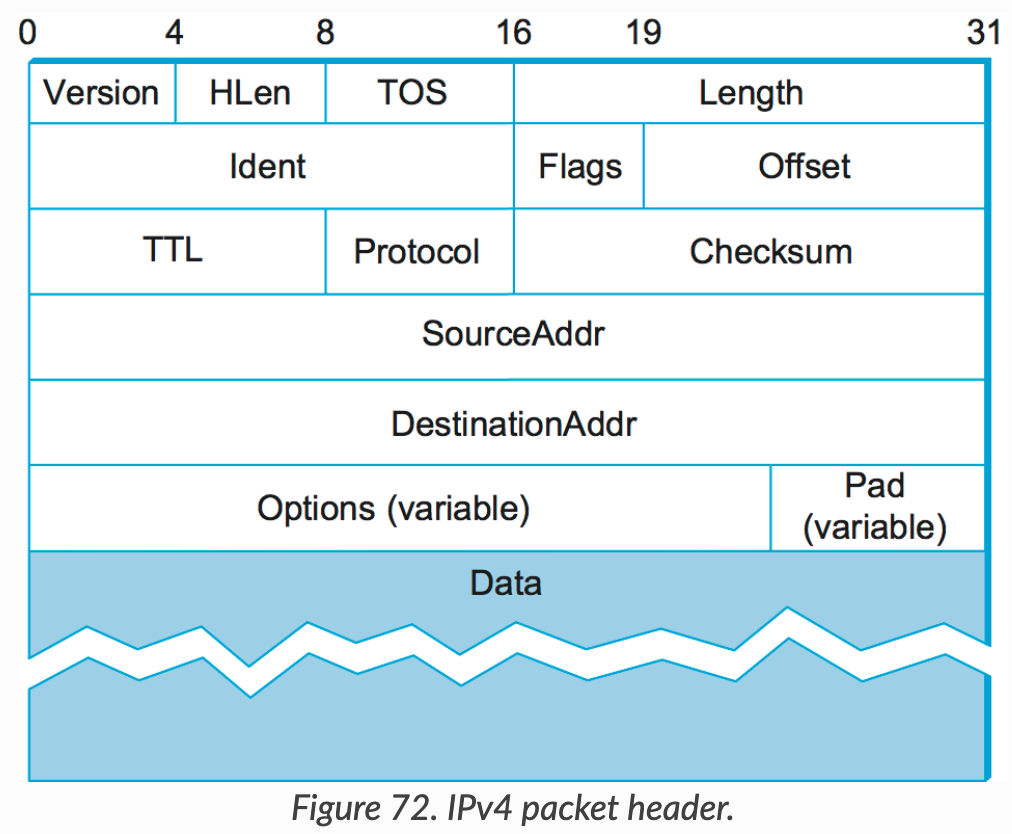
\includegraphics[scale=0.4]{IPv4PacketHeader}
  \end{center}
  Looking at the various IP header fields:
  \begin{itemize}
    \item \textbf{Version}: specifies which version of IP is being used. 
    \item \textbf{Hlen}: specifies the length of the header in 32-bit words.
    \item \textbf{TOS}: type of service. Allows packets to be treated differently based on application needs.
    \item \textbf{Length}: size of entire packet (including header) as bytes.
    \item Note that the second word is used for fragmentation and reassembly (explained below)
    \item \textbf{TTL}: time to live (used to discard packets that have been stuck in the routing loop)
    \item \textbf{Protocol}: demultiplexing key used to identify which higher protocol to send to (UDP, TCP)
    \item \textbf{Checksum}: used to check for bit corruption in the header
    \item \textbf{SourceAddr}: which address packet came from (allows recipients decide if they want to accept)
    \item \textbf{DestinationAddr}: which address packet is sent to
    \item \textbf{Options}: additional options may be added (can be determined using \textbf{HLen})
  \end{itemize}
  \subsubsection{Fragmentation and Reassembly}
  Biggest issue is that each network technology has its own idea of how large a packet is. Thus, packets must be fragmented and reassembled when they don't fit in the network technology. \\ \\
  Fragmentation occurs when a router receives a datagram that it wants to forward over the network with a lower MTU. The receiving host will recognize which fragments belong together through its \textbf{Ident} header field. If all fragments don't arrive, the host discards the packet entirely and does not attempt recover missing fragments. \\ \\
  The \textbf{Flag} header field is used to indicate that there are more packets coming. The \textbf{Offset} header field is used to identify which partition of the packet is being sent over.
  \subsection{Global Addresses}
  IP addresses are \textbf{hierarchical}, consisting of a \textbf{network} part (identifies the network thae host is attached to) and a \textbf{host} part (unique host on the network). Addresses are written as 4 octets, or \textbf{dotted quad} notation and can be broken down into 5 classes subnets, in the classical model:
  \begin{itemize}
    \item A: $0-127.y.x.w$ $\quad 0, \underbrace{7b}_{\text{network}}, \underbrace{24b}_{\text{host}}$
    \item B: $128 - 191.y.x.w$ $\quad 10, \underbrace{14b}_{\text{network}}, \underbrace{16b}_{\text{host}}$
    \item C: $192-223.y.x.w$ $\quad 110, \underbrace{21b}_{\text{network}}, \underbrace{8b}_{\text{host}}$
    \item D: $224-239.y.x.w$
    \item D: $240-255.y.x.w$
  \end{itemize}
  Classical representation runs out of space rapdily so we can instead break larger subnets into smaller subnets using a \textbf{network mask} (e.g. $255.255.0.0$). Then:
  \[\text{mask } \& \text{ address} = 128.8.0.0 \text{ base address }\]
  \subsection{Datagram Forwarding in IP}

\end{document}
